\documentclass{patmorin}

\usepackage{amssymb,amsthm,amsmath}
\usepackage{url,html}
\usepackage[longnamesfirst,numbers,sort&compress]{natbib}
\usepackage{cleveref}
\usepackage{paralist}
\usepackage{todonotes}
\usepackage[noend]{algorithmic}

\setlength{\parskip}{1ex}

\newcommand{\pref}[1]{(P\ref{#1})}
\newcommand{\psref}[1]{(P\ref{#1}$^{\star}$)}

\newcommand{\R}{\mathbb{R}}
\newcommand{\N}{\mathbb{N}}

\newtheorem{lemma}{Lemma}
\newtheorem{theorem}{Theorem}

\title{\MakeUppercase{Sparse Induced-Universal Graphs for Planarity}}
\author{Louis Esperet, Gwenaël Joret, and Pat Morin}

\begin{document}

\maketitle

\begin{abstract}
    We show that, for $n\in\N$, there exists a graph $U_n$ with $n^{1+o(1)}$ vertices and edges such that, for any $n$-vertex planar graph $G$, $U_n$ contains an induced subgraph isomorphic to $G$.  This result extends to other graph families having a product structure theorem, including bounded genus graphs, apex-minor-free graphs, bounded-degree graphs from minor-closed families, and $k$-planar graphs for constant $k$.
\end{abstract}

\section{Introduction}

Very recently, \citet{dujmovic.esperet.ea:adjacency} described a $(1+o(1))\log n$-bit adjacency labelling scheme for planar graphs.  This means that there is a single function $A:\{0,1\}^*\times\{0,1\}^* \to\{0,1\}$ such that, for any $n$ vertex planar graph $G$ there is a labelling $\ell:V(G)\to\{0,1\}^{(1+o(1))\log n}$ for which $A(\ell(v),\ell(w))=1$ if and only if $vw\in E(G)$.

This result has the following immediate consequence: For every positive integer $n$, there exists a graph $I_n$ having $n^{1+o(1)}$ \emph{vertices} such that, for every $n$-vertex planar graph $G$, $I_n$ contains an induced subgraph isomorphic to $G$.  To see this, let $I_n$ be the graph with vertex set $V(I_n):=\{0,1\}^{(1+o(1))\log n}$ and for which $xy\in E(I_n)$ if and only $A(x,y)=1$.  Then, for any $n$-vertex planar graph $G$ with labelling $\ell$, the induced subgraph $I_n[\{\ell(v):v\in V(G)\}]$ is isomorphic to $V(G)$.  The graph $I_n$ is called an \emph{induced-universal graph} for the class of $n$-vertex planar graphs.

Using one of the main ideas from \cite{dujmovic.esperet.ea:adjacency}, \citet{esperet.joret.ea:sparse} showed that there exists a graph $S_n$ with $n^{1+o(1)}$ \emph{edges} such that, for every $n$-vertex planar graph $G$, $S_n$ contains a subgraph (not necessarily induced) isomorphic to $G$.  The graph $S_n$ is called a \emph{subgraph-universal graph} for the class of $n$-vertex planar graphs.

Notice the contrasts between these two results: $I_n$ contains every $n$-vertex planar graph $G$ as an \emph{induced} subgraph whereas $S_n$ may only contain $G$ as a subgraph but not an induced subgraph.  Note that these two notions are very different: $K_n$ contains every at most $n$-vertex graph as a subgraph, but only contains cliques as induced subgraphs. On the other hand, the graph $S_n$ is sparse, having only $n^{1+o(1)}$ edges whereas $I_n$ has $n^{1+o(1)}$ vertices and may have have $n^{2+o(1)}$ edges.

In this paper we show that there exists \emph{sparse} \emph{induced}-universal graphs for planarity:

\begin{theorem}\label{main-planar}
    For every $n\in\N$, there exist a a graph $U_n$ having $n^{1+o(1)}$ edges and vertices and such that, for every $n$-vertex planar graph $G$, $U_n$ contains an induced subgraph isomorphic to $G$.
\end{theorem}

The remainder of this paper is organized as follows. In \cref{review} we review the adjacency labelling scheme of \cite{dujmovic.esperet.ea:adjacency} that is the starting point for this work and argue that this labelling scheme does not produce a sparse induced-universal graph $I_n$.  In \cref{modifications} we describe a non-trivial modification of this labelling scheme and show that this modification of the labelling scheme does produce a sparse induced-universal graph $U_n$ that proves \cref{main-planar}.  \Cref{summary} summarizes and concludes.



\section{Review of Adjacency Labelling}
\label{review}

We now summarize review the most relevant aspects of the adjacency labelling scheme of \citet{dujmovic.esperet.ea:adjacency}.  For any integer $t\ge 1$, let $\mathcal{G}_t$ the set of graphs that contains, for every $t$-tree $H$ and every path $P$, every subgraph of $H\boxtimes P$.  The labelling scheme of \citet{dujmovic.esperet.ea:adjacency} works any $n$-vertex member of $\mathcal{G}_t$ for any constant $t$.  In particular, it works for any $n$-vertex planar graph because $\mathcal{G}_8$ contains every planar graph \cite{X}.

We now describe how the labelling scheme works for some $n$-vertex member $G$ of $\mathcal{G}_t$, so $G$ is a subgraph of $H\boxtimes P$ for some $t$-tree $H$ and some path $P$.  Without loss of generality, we may assume that the vertices of $P$ are the integers $1,\ldots,h$ in the order they occur on the path $P$ and that, for each $y\in\{1,\ldots,h\}$ there exists at least one $v\in V(H)$ such that $(v,y)\in V(G)$.

Without loss of generality, we may assume that $H$ has at least $t+1$ vertices. Fix a tree decomposition $(B_x:x\in V(T))$ of $H$ in which each bag has size exactly $t+1$ and in which no two bags have the same contents.  Root $T$ at an arbitrary node $r$ and, for each vertex $v$ of $H$, let $C_v:=B_x$ where $x$ is the minimum-depth node of $T$ such that $v\in B_x$.  The vertex set $C_v$ has size $t+1$, includes $v$ and is called the \emph{family clique} of $v$.

Each vertex $w\in C_v$ is called an \emph{$H$-parent} of $v$.  Fix a proper colouring $\varphi:H\to\{1,\ldots,t+1\}$.  For any vertex $v$ of $H$, the \emph{$i$-parent} $p_i(v)$ of $v$ is the unique node $w\in C_v$ with $\varphi(w)=i$.  Note that $v$ is and $H$-parent of itself and, specifically, $v$ is the $\varphi(v)$-parent of itself.

The scheme makes use of binary search trees.\todo{Define BST}  For any node $x$ in a binary search tree $T$, $\sigma_T(x)$ is the binary string $b_1,\ldots,b_k$ obtained by from the root-to-$x$ path $x_0,\ldots,x_k$ in $T$ by setting $b_i=0$ or $b_i=1$ depending on whether $x_i$ is the left or right child of $x_{i-1}$, respectively. Note that the function $\sigma_T:V(T)\to\{0,1\}^*$ is injective.  We extend this notation to paths so that, if $P$ is a path from the root of $T$ to some node $x$, then $\sigma_T(P):=\sigma_T(x)$.


The scheme also makes use an interval supergraph of $H$.  Each vertex $v$ of $H$ is mapped to a real interval $[a_v,b_v]$ in such a way that $vw\in E(H)$ implies that $[a_v,b_v]\cap [a_w,b_w]\neq\emptyset$.  This mapping is also thin, in the following sense:

\begin{compactenum}[(P1)]
    \item for any $x\in \R$, $|\{v\in V(H): x\in[a_v,b_w]\}|\in O(t\log n)$.\label{thin}
\end{compactenum}

For each $y\in\{0,\ldots,n+1\}$, let $L_y:=\{v\in V(H): (v,y)\in V(G)\}$ and let $S_y:=\bigcup_{v\in L_y}C_v$.  The labelling scheme first finds sets $S^+_1,\ldots,S^+_h$ of total size $O(n)$ such that $S^+_y\supseteq S_{y-1}\cup S_y\cup S_{y+1}$.\footnote{The original labelling scheme only uses $S^+_y\supseteq S_{y-1}\cup S_y$ but it is convenient for us to include $S_{y+1}$ as well and this change does not invalidate anything in the original scheme.}

\citet{dujmovic.esperet.ea:adjacency} define a sequence of binary search trees $T_1,\ldots,T_h$ such that, for each $y\in\{1,\ldots,h\}$ and each $v\in S^+_y$, $T_y$ contains at least one value $x\in [a_v,b_v]$.  This leads to the following crucial definition: For each $v\in S^+_y$, $x_{y}(v)$ is the minimum-depth node $x$ of $T_y$ such that $x\in [a_v,b_v]$. Note that $x_y(v)$ is well-defined since $T_y$ contains at least one node $x\in[a_v,b_v]$.   The following property follows from these definitions and Helly's Theorem:

\begin{compactenum}[(P1)]\setcounter{enumi}{1}
    \item For any $v\in L_y$, there exists a path $P_y(v)$ that begins at the root of $T_y$ and contains every node in $X_y(v):=\{x_{y}(w): w\in C_v\}$.\label{clique-path}
\end{compactenum}

For each $y\in\{1,\ldots,h\}$ and each $v\in L_y$, we define $P_y(v)$ to be the minimum length path in $T_y$ that satisifies \pref{clique-path}, so that $P_y(v)$ begins at the root of $T$ and ends at the node in $X_y(v)$ of maximum $T_y$-depth. For each $y\in\{1,\ldots,h\}$ and each $x\in V(T_y)$, $d_y(x)$ denote the depth of $x$ in the tree $T_x$.

It is helpful to think of $x_y$ as a function $x_y:S^+_y\to V(T_y)$.  For each $y\in\{1,\ldots,h\}$ and each node $x$ of $T_y$, let $B_x:=\{v\in S^+_y: x_y(v)=x\}=x_y^{-1}(x)$.\todo{Should we use $B_{y,x}$?}  Since $x\in[a_v,b_v]$ for each $v\in B_x$, \pref{thin} implies the following property:

\begin{compactenum}[(P1)]\setcounter{enumi}{2}
    \item For each $y\in\{1,\ldots,h\}$ and each $x\in V(T_y)$, $|B_x|\in O(t\log n)$. \label{small-bags-i}
\end{compactenum}

Let $\psi_y:S^+_y\to\{1,\ldots,O(t\log n)\}$ be a colouring of $S^+_y$ such that, for each $x\in V(T)$ and each distinct pair $v,w\in B_x$ $\psi_y(v)\neq\psi_y(w)$.  Such a colouring exists by \pref{small-bags-i} and because $x_y$ is a function so each $v\in S^+_y$ appears in $B_x$ for exactly one $x\in V(T)$.  Note that, for any $v\in S^+_y$, the pair $(x_y(v), \psi_y(v))$ uniquely identifies $v$.  Since the signature function $\sigma_y$ is injective, this means that $\sigma_y(x_y(v))$ and $\psi_y(v)$ also uniquely identify $v$.

\begin{compactenum}[(P1)]\setcounter{enumi}{3}
    \item For any $y\in\{1,\ldots,h\}$ and any distinct $v,w\in S^+_h$, $\sigma_y(x_y(v))\neq \sigma_y(x_y(x)) $ or $\psi_y(v)\neq\psi_y(w)$.\label{unique-match}
\end{compactenum}

The binary search tree sequence $T_1,\ldots,T_h$ is very special because it has two important properties:
\begin{compactenum}[(P1)]\setcounter{enumi}{4}
    \item For each $y\in\{1,\ldots,h\}$, $h(T_y)\le \log|S^+_y|+o(\log n)$.
    \item There exists a universal function $J:\{0,1\}^*\times\{0,1\}^*\to\{0,1\}^*$ such that for each $y\in\{1,\ldots,h-1\}$ and each $x\in V(T_y)\cap V(T_{y+1})$ there exists a bitstring $\mu_y(x)$ of length $o(\log n)$ such that $J(\sigma_{T_y}(x),\mu_y(x))=\sigma_{T_{y+1}}(x)$.
\end{compactenum}
The bitstring $\mu_y(x)$ is called a \emph{transition code}.  The existence of the tree sequence $T_1,\ldots,T_h$ and corresponding transition codes is non-trivial and is the primary technical tool used to establish the results in \cite{dujmovic.esperet.ea:adjacency,esperet.joret.ea:sparse}.

\subsection{The Labels}
\label{labels-i}

For each vertex $(v,y)$ of $G$, the label $\ell(v,y)$ has these parts:

\begin{compactenum}[(L1)]
    \item $\alpha(y)$: a bitstring of length of $\log n-\log |S^+_y|+o(\log n)$.  Given $\alpha(y_1)$ and $\alpha(y_2)$ it is possible to distinguish between the following cases:
    \begin{inparaenum}
        \item $y_1=y_2$;
        \item $y_1=y_2+1$;
        \item $y_1=y_2-1$;
        \item $|y_1-y_2|\ge 2$.
    \end{inparaenum}

    \item $\sigma_y(P_y(v))$: this is a bitstring of length at most $h(T_y)\le \log|S^+_y| + o(\log n)$
    % a bitstring of length at most $h(T_y)$ that encodes the path $P_y(v)$ where a 0 (respectively, 1) indicates a step from the current node to its left (respectively, right) child.

    \item $\mu_y(v)$: a bitstring of length $o(\log n)$.  This bitstring is designed so that, for any node $v\in S^+_y\cap S^+_{y+1}$, it is possible to recover $\sigma_{y+1}(P_{y+1}(v))$ given only $\sigma_y(P_y(v))$ and $\mu_y(v)$.

    \item $\varphi(v)$: the colour of $v$ in the proper colouring of $H$ (a bitstring of length $\lceil\log(t+1)\rceil$).

    \item $d_y(x_y(p_i(v)))$ for each $i\in\{1,\ldots,t+1\}$ (a bitstring of length $(t+1)\lceil\log(t+1)\rceil$).

    \item $\psi_{y+b}(p_i(v))$ for each $i\in\{1,\ldots,t+1\}$ and each $b\in\{-1,0,1\}$ (a bitstring of length $O(t\log\log n + t\log t)$).\label{psi}

    \item $a_y(v)$: A bitstring of length $3(t+1)$ that indicates, for each $i\in\{1,\ldots,t+1\}$ and each $b\in\{-1,0,1\}$ whether $G$ contains the edge with endpoints $(v,y)$ and $(p_i(v),y+b)$.
\end{compactenum}

The label (L1) requires some further explanation. $\alpha(y)$ consists of two parts: $(\alpha_1(y))$ is a bitstring of length at most $\log n-\log |S^+_y|$ and $\alpha_2(y)$ is a bitstring of length at most $\log\log n+O(1)$.  These strings are designed so that there is a universal function $N$ such that $N(\alpha(y_1))=\alpha_1(y_2)$ if and only if $y_2=y_1+1$.  Clearly this make it possible to distinguish between cases~(a)--(d).  It also has the following implication:  For any fixed $\alpha(y_1)$ there are at most $2^{\log \log n+O(1)}=O(\log n)$ values of $\alpha(y_2)$ that fall into case (b).  Indeed, these are $D(\alpha(y_1)):=\{N(\alpha(y_1))\mathbin{\circ} s: s\in\{0,1\}^{\log\log n}\}$.

\subsection{Adjacency Testing}

Given inputs $\ell(v_1,y_1)$ and $\ell(v_2,y_2)$, the adjacency testing function $A$ works as follows:
\begin{enumerate}
    \item Using $\alpha(y_1)$ and $\alpha(y_2)$, determine which of the following cases applies:
    \begin{enumerate}[(a)]
        \item $y:=y_1=y_2$.  For each $i\in\{1,\ldots,t+1\}$, determine if $v_1=p_i(v_2)$ (or \textit{vice-versa}) and, if so, use $a_y(v_2)$ (or $a_y(v_1)$, respectively) to determine if $(v_1,y)$ and $(v_2,y)$ are adjacent in $G$. Specifically, if $v_1=p_i(v_2)$ then one of the bits in $a_y(v_2)$ indicates whether or $(v_1,y_1)$ and $(v_2,y_1)$ are adjacent in $G$. If $v_1\neq p_i(v_2)$ and $v_2\neq p_i(v_1)$ for every $i\in\{1,\ldots,h\}$, then $v_1v_2\not\in E(H)$ and hence $(v_1,y)$ and $(v_2,y)$ are not adjacent in $G\subseteq H\boxtimes P$.

        By \pref{unique-match}, testing if $v_1=p_i(v_2)$, is equivalent to testing if $\sigma_y(x_y(v_1))=\sigma_y(x_y(p_i(v_2)))$ and $\psi_y(v_1)=\psi_y(p_i(v_2))$. We now show that $\ell(v_1,y_1)$ and $\ell(v_2,y)$ contain enough information to perform this test.
        \begin{compactitem}
            \item We can recover $d_y(x_y(v_1))=d_y(x_y(p_{\varphi(v_1)}(v_1)))$ and using this, recover $\sigma_y(x_y(v_1))$ from $\sigma_y(P_y(v_1))$ and $d_y(x_y(v_1))$.  Next, we can recover $\sigma_y(x_y(p_i(v_2)))$ from $\sigma_y(P_y(v))$ and $d_y(x_y(p_i(v)))$. This makes it possible to test if $\sigma_y(x_y(v_1))=\sigma_y(x_y(p_i(v_2)))$.
            \item  The colour $\psi_y(v_1)$ can be recovered from the label of $(v_1,y_1)$ since $\psi_y(v_1)=\psi_y(p_{\varphi(v_1)}(v_1))$.  The colour $\psi_y(p_i(v_2))$ is stored explicitly in the label of $(v_2,y_2)$.  This makes it possible to test if $\psi_y(v_1)=\psi_y(p_i(v_2))$.
        \end{compactitem}
        \item $y:=y_2=y_1+1$.  In this case, recover $\sigma_y(P_y(v_1))$ from $\sigma_{y_1}(P_{y_1}(v_1))$ and $\mu_{y_1}(v_1)$.  At this point, the algorithm proceeds exactly as in the previous case except that, in the final step one bit of $a_{y_2}(v_2)$ is used to check if $(v_1,y_1)=(p_i(v_2),y_2-1)$ is present in $G$.

        \item $y:=y_1=y_{2+1}$. This case is symmetric to the previous case with the roles and $1$ and $2$ reverse.

        \item $|y_1-y_2|\ge 2$.  In this case $y_1\neq y_2$ and $y_1y_2\not\in E(P)$ and therefore $(v_1,y_1)$ and $(v_2,y_2)$ are not adjacent in $G\subseteq H\boxtimes P$.
    \end{enumerate}
\end{enumerate}

\subsection{Edge Density of the Universal Graph}
\label{density-lower-bound}

We now explain why the universal graph $I_n$ defined by the preceding labelling scheme is not sparse.  The main issue is the definition of $P_y(v)$ as the path in $T_y$ that contains every node in $X_y(v):=\{x_y(w):w\in C_v\}$.  The problem comes from the fact that there can be nodes in $X_y(v)$ that have much greater $T_y$-depth than $x_y(v)$.  This ultimately leads to a large complete bipartite graph with sides $L$ and $R$ in which the elements of $L$ all correspond to a single vertex $(v,y)$ of $H\boxtimes P$.

Consider a set of subgraphs $G_1,\ldots,G_k$ of $H\boxtimes P$ that each contain the vertices $(v_0,y),\ldots,(v_k,y)$ and the edges $(v_0,y)(v_i,y)$ for each $i\in\{1,\ldots,k\}$.  Each of these graphs has a labelling scheme in which the vertices of $G_i$ are labelled by a function $\ell_i:V(G_i)\to\{0,1\}^{(1+o(1))\log n}$.  We add an additional subscript, $i$, to all of our notations so that, for example $\sigma_{i,y}(P_{i,y}(v))$ is the part of the label corresponding to $\sigma_y(P_y(v))$ in the labelling $\ell_i$ for $G_i$.

Suppose that, for each $i,j\in\{1,\ldots,k\}$, $\sigma_{i,y}(x_{i,y}(v_0))=\sigma_{j,y}(x_{j,y}(v_0))$ but that $\sigma_{i,y}(P_{i,y}(v_0))\neq\sigma_{j,y}(P_{j,y}(v_0))$.  This just means that, the path from the root is $T_{i,y}$ to $x_{i,y}(v_0)$ is the same for each $i\in\{1,\ldots,k\}$, but the path from $x_{i,y}(v_0)$ to the deepest node in $X_{i,y}$ is different for each $i\in\{1,\ldots,k\}$.  There is nothing about the definition of the labelling scheme that rules out this possibility.  Indeed, it could be that $x_{i,y}(v_0)$ is the root of $T_{i,y}$ for each $i\in\{1,\ldots,k\}$, in which case there is no apriori reason to believe that, for distinct $i,j\in\{1,\ldots,k\}$ that $\sigma_{i,y}(P_{i,y}(v_j))=\sigma_{i,y}(P_{i,y}(v_j))$.  In fact, this seems unlikely.

Therefore, the universal graph $I_n$ contains $k$ distinct vertices $z_1,\ldots,z_k$ each corresponding to $(v_0,y)$ where $z_i=\ell_i(v_0,y)$ is the node corresponding to $(v_0,y_0)$ in the graph $G_i$.  For each $i\in\{1,\ldots,k\}$, $I_n$ also contains $k$ distinct vertices $z_{i,j}=\ell_i(v_j,y)$.  Since $(v_0,y)$ is adjacent to $(v_i,y)$ for each $i\in\{1,\ldots,k\}$, $z_i$ is adjacent to $z_{i,k}$ and therefore $z_i$ has degree at least $k$. Since this is true for each $i\in\{1,\ldots,k\}$, we conclude that, in this example, $I_n$ has at least $k^2$ edges.  Finally, note that there is no sublinear upper bound on $k$. Indeed, it is conceivable that this situation occurs even with $k=n/2$, yielding a universal graph $I_n$ with $\Omega(n^2)$ edges.

\todo[inline]{The preceding example uses a high-degree vertex $v_0$, but the same problem exists if the graph has bounded degree (in fact, even if the graph is a path).  I think the example in \cref{bad-example} might be the most compelling, though since, for that one, it looks like any easy fix would be hack that doesn't generalize.}

\begin{figure}
    \begin{center}
        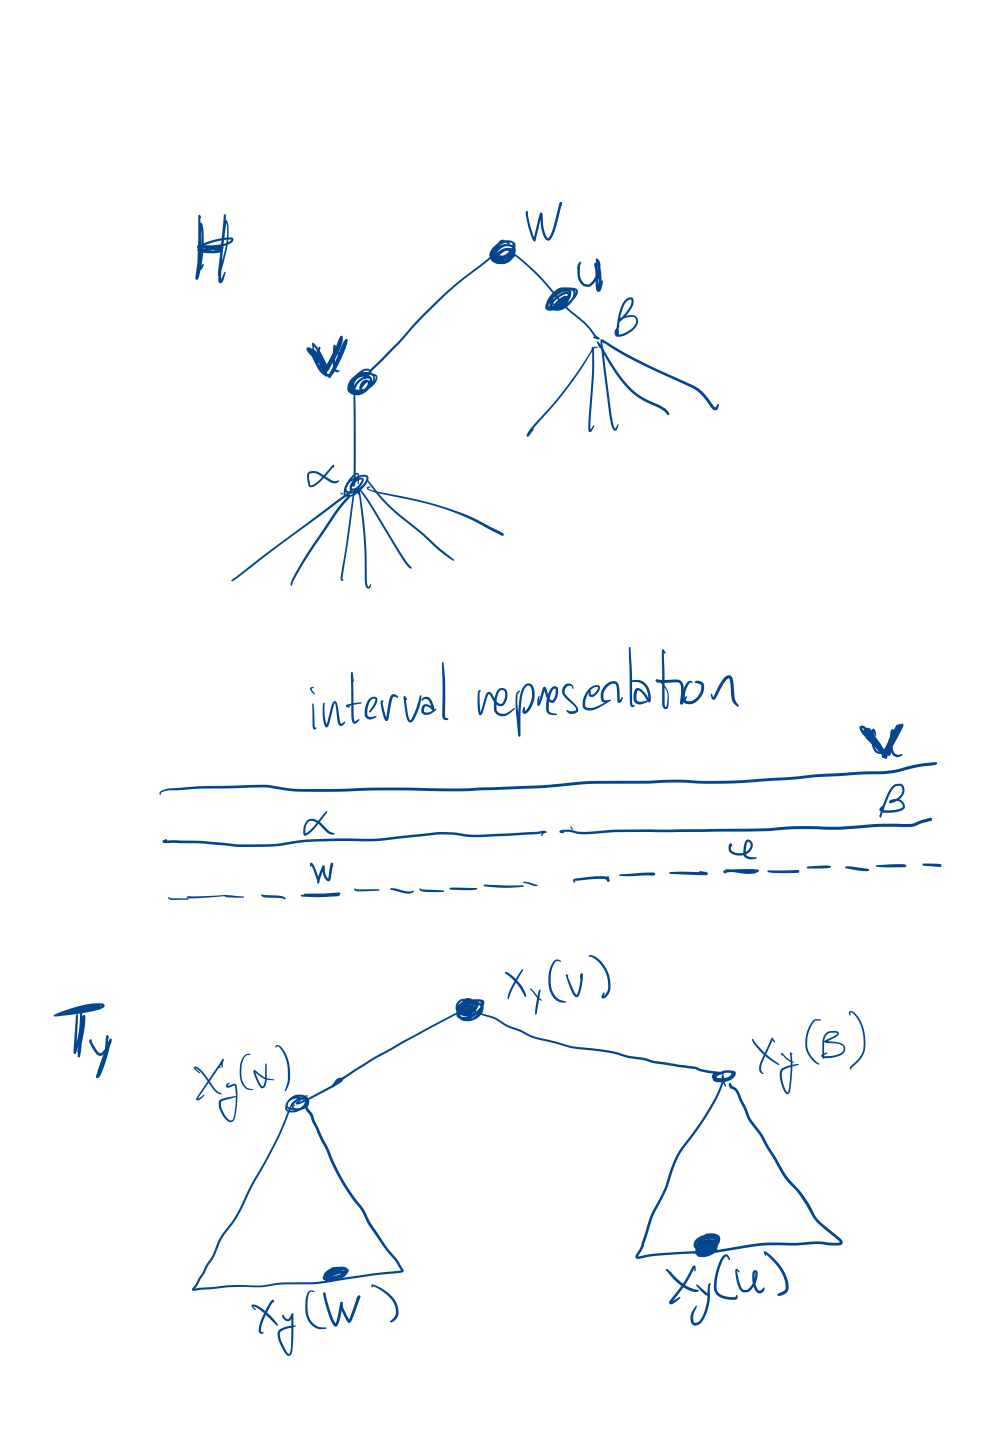
\includegraphics[width=.5\textwidth]{figs/bad-example}
    \end{center}
    \caption{A better bad example}
    \label{bad-example}
\end{figure}

\section{A Sparse Universal Graph}
\label{modifications}

We now describe how to modify the adjacency labelling scheme of \citet{dujmovic.esperet.ea:adjacency} so that the resulting universal subgraph is sparse.  As discussed above, the main obstacle comes from the fact that some vertex $(v,y)$ can have an $i$-parent $w:=p_i(v)$ such that $x_y(w)$ has $T_y$-depth much greater than $x_y(v)$.  In order to avoid this, we modify the function $x_y:S^+_y\to V(T_y)$ to create a new function $x'_y$ that avoids this. Initially $x'_y(v)=x_y(v)$ for each $v\in S^+_y$, but then modifications are performed by calling the following recursive procedure with the root of $T_y$ as its argument:

\noindent
\begin{minipage}{\textwidth}
    $\textsc{Fixup}(x)$:
    \begin{algorithmic}[1]
        \FOR{each $v\in V(H)$ such that $x'_y(v)=x$}
            \FOR{each $w\in C_v \cap S^+_y$}
                \IF{$d_y(x'_y(w)) > d_y(x)+1$}
                    \STATE{\COMMENT{make $x'_y(w)$ is a child of $x=x'_y(v)$}}
                    \STATE{$x'_y(w)\gets\mbox{the depth-$(d_y(x)+1)$ $T_y$-ancestor of $x'_y(w)$}$ \label{changes}}
                \ENDIF
            \ENDFOR
        \ENDFOR
        \STATE{\textsc{Fixup}(left child of $u$) (if any)}
        \STATE{\textsc{Fixup}(right child of $u$) (if any)}
    \end{algorithmic}
\end{minipage}

% Let $x_y$ denote the original function $x_y:S^+_y\to V(T_y)$ used by \citet{dujmovic.esperet.ea:adjacency} and let $x'_y:S^+_y\to V(T_y)$ denote the new function obtained after running $\textsc{Fixup}(r)$ on the root $r$ of $T_y$.

Observe that the only modifications to $x'_y$ that occur do so in Line~\ref{changes} and they involve setting $x'_y(w)$ to an ancestor of $x_y(w)$.  Therefore, for any vertex $v\in S^+_y$, $x'_y(v)$ is a $T$-ancestor of $x_y(v)$.  This immediately implies that that, after running $\textsc{Fixup}(r)$, \pref{clique-path} still holds. Indeed, the same path $P_y(v)$ contains every node in $X_y(v)$.

However, it is not the case that $x'_y$ satisfies \pref{small-bags-i}.  Indeed, $B'_x:=\{v\in S^+_y: x'_y(v)=x\}$ can be much larger than $B_x$ and, even larger than $O(t\log n)$.  The next lemma shows that the size of $B'_x$ is still polylogarithmic in $n$.

\begin{lemma}\label{small-bags-ii-lem}
    For each $y\in\{1,\ldots,h\}$ and each node $x$ of $T_y$, $|B'_x|\in O(t(\log n)^{t+2})$.
\end{lemma}

\begin{proof}
    Let $x$ be some node of $T_y$ and suppose that, for some $w\in S^+_y$ $x'_T(w)=x$.  We can trace $w$ back through a path $w_0,w_1,w_2,..,w_d$ in $H$ such that
    \begin{compactenum}[(a)]
        \item $w_0=w$;
        \item $w_{i-1}$ is an $H$-parent of $w_i$ for each $i\in\{1,...,d\}$;
        \item $x'_y(w_{i})$ is the $T_y$-parent of $x'_y(w_{i-1})$ for each $i\in\{1,...,d\}$; and
        \item $x_T(w_d)=x'_T(w_d)$.
    \end{compactenum}
    In particular $w$ is an $H$-ancestor of $w_d$ and there is a path $w_0,\ldots,w_d$ in $H$ of length at most $d$ between with endpoints $w$ and $w_d$.  In the language of \citet{pilipczuk.siebertz:polynomial} $w_0$ is \emph{$d$-reachable} from $w_d$.  \citet[Lemma~13]{pilipczuk.siebertz:polynomial-arxiv} shows that the number of $d$-reachable $H$-ancestors for any node $v$ in a $t$-tree $H$ is at most $\binom{d+t}{t}$.

    Now, let $x=x_0\ldots,x_k$ be the path from $x=x_0$ to the root $x_k$ of $T_y$. By the preceding argument, for each $v\in B'_x$ there exists some $d\in\{0,\ldots,k\}$ such that $w$ is a $d$-reachable $H$-ancestor of some node $v\in B_{x_d}$.  It follows that
    \[
        |B'_x|
            \le \sum_{d=0}^k |B_{x_d}|\binom{t+d}{t}
            \in O(tk^{t+1}\log n)
            \subseteq O(t(\log n)^{t+2}) \enspace . \qedhere
    \]
\end{proof}

Therefore, by \cref{small-bags-ii-lem}, the modified labelling scheme satisfies the following weakening of \pref{small-bags-i}:

\begin{compactenum}[(P1$^{\star}$)]\setcounter{enumi}{2}
    \item $|B'_x|\in O(t(\log n)^{t+2})$. \label{small-bags-ii}
\end{compactenum}

Therefore, the labelling scheme obtained with the modified definition of $x_y$ satisfies \pref{thin}, \pref{clique-path} (with $x_y$ replaced by $x'_y$), and \psref{small-bags-ii}.

\subsection{The New Labels}

For each $y\in\{1,\ldots,h\}$ and each $v\in S^+_y$, we define $X'_y(v)=\{x'_y(w): w\in C_v\}$ and $P'_y(v)$ as the shortest path that begins at the root of $T_y$ and contains every node $X'_y(v)$.  Let $\psi'_y:S^+_y\to\{1,\ldots,O(t(\log n)^{t+2})\}$ be a colouring of $S^+_y$ such that, for each $x\in V(T)$ and each distinct pair $v,w\in B'_x$ $\psi(v)\neq\psi(w)$.  For each vertex $(v,y)$ of $G$, the label $\ell(v,y)$ has these parts:

\begin{compactenum}[(NL1)]
    \item $\alpha(y)$: this is the unmodified from the original scheme.

    \item $\sigma_y(x_y(v))$: note that this is not $\sigma_y(P'_y(v))$, but
    $\sigma_y(x'_y(v))$ can be recovered from $\sigma_y(x_y(v))$ and $d_y(x'_y(p_{\varphi(v)}(v))$. This makes it possible to recover $\sigma_y(P'_y(v))=\sigma_y(x'_y(v))\mathbin{\circ} b_y(v)$ where $b_y(v)$ is defined in (NL8), below.

    \item $\mu'_y(v)$: a bitstring of length $o(\log n)$.  This bitstring is designed so that, for any node $v\in S^+_y\cap S^+_{y+1}$, it is possible to recover $\sigma_{y+1}(x_{y+1}(v))$ given only $\sigma_y(x_y(v))$ and $\mu_y(v)$.\footnote{The \emph{transition code} $\mu'_y(v)$ is defined in \cite[Section~5.3]{dujmovic.esperet.ea:adjacency}.}

    \item $\varphi(v)$: the colour of $v$ in the proper colouring of $H$ (a bitstring of length $\lceil\log(t+1)\rceil$).

    \item $d_y(x'_y(p_i(v)))$ for each $i\in\{1,\ldots,t+1\}$ (a bitstring of length $(t+1)\lceil\log(t+1)\rceil$).

    \item $\psi'_{y+b}(p_i(v))$ for each $i\in\{1,\ldots,t+1\}$ and each $b\in\{-1,0,1\}$ (a bitstring of length $O(t\log\log n)$).\label{psi-prime}

    \item $a_y(v)$: this is unmodified from the original scheme.

    \item $b_y(v)$: A binary string of length at most 1 such that $\sigma_y(P'_y(v))=\sigma_y(x'_y(v))\mathbin{\circ}b_y(v)$.
\end{compactenum}

\subsection{Adjacency Testing}

Given inputs $\ell(v_1,y_1)$ and $\ell(v_2,y_2)$, the adjacency testing function $A$ for the new labelling scheme works as follows:
\begin{enumerate}
    \item Using $\alpha(y_1)$ and $\alpha(y_2)$, determine which of the following cases applies:
    \begin{enumerate}[(a)]
        \item $y:=y_1=y_2$.  For each $i\in\{1,\ldots,t+1\}$, determine if $v_1=p_i(v_2)$ (or \textit{vice-versa}) and, if so, use $a_y(v_2)$ (or $a_y(v_1)$, respectively) to determine if $(v_1,y)$ and $(v_2,y)$ are adjacent in $G$. Specifically, if $v_1=p_i(v_2)$ then one of the bits in $a_y(v_2)$ indicates whether or $(v_1,y_1)$ and $(v_2,y_1)$ are adjacent in $G$. If $v_1\neq p_i(v_2)$ and $v_2\neq p_i(v_1)$ for every $i\in\{1,\ldots,h\}$, then $v_1v_2\not\in E(H)$ and hence $(v_1,y)$ and $(v_2,y)$ are not adjacent in $G\subseteq H\boxtimes P$.

        By \pref{unique-match}, testing if $v_1=p_i(v_2)$, is equivalent to testing if $\sigma_y(x'_y(v_1))=\sigma_y(x'_y(p_i(v_2)))$ and $\psi'_y(v_1)=\psi'_y(p_i(v_2))$. We now show that $\ell(v_1,y_1)$ and $\ell(v_2,y)$ contain enough information to perform this test.
        \begin{compactitem}
            \item We can recover $d_y(x'_y(v_1))=d_y(x'_y(p_{\varphi(v_1)}(v_1)))$ and using this, recover $\sigma_y(x'_y(v_1))$ from $\sigma_y(x_y(v_1))$ and $d_y(x'_y(v_1))$.  Next, we can recover $\sigma_y(x'_y(p_i(v_2)))$ from $\sigma_y(P'_y(v))$ and $d_y(x'_y(p_i(v)))$. This makes it possible to test if $\sigma_y(x'_y(v_1))=\sigma_y(x'_y(p_i(v_2)))$.
            \item  The colour $\psi'_y(v_1)$ can be recovered from the label of $(v_1,y_1)$ since $\psi'_y(v_1)=\psi'_y(p_{\varphi(v_1)}(v_1))$.  The colour $\psi'_y(p_i(v_2))$ is stored explicitly in the label of $(v_2,y_2)$.  This makes it possible to test if $\psi'_y(v_1)=\psi'_y(p_i(v_2))$.
        \end{compactitem}

        \item $y:=y_2=y_1+1$.  In this case, recover $\sigma_y(x_y(v_1))$ from $\sigma_{y_1}(x_{y_1}(v_1))$ and $\mu'_{y_1}(v_1)$.  At this point, the algorithm proceeds exactly as in the previous case except that, in the final step one bit of $a_{y_2}(v_2)$ is used to check if $(v_1,y_1)=(p_i(v_2),y_2-1)$ is present in $G$.

        \item $y:=y_1=y_{2+1}$. This case is symmetric to the previous case with the roles and $1$ and $2$ reverse.

        \item $|y_1-y_2|\ge 2$.  In this case $y_1\neq y_2$ and $y_1y_2\not\in E(P)$ and therefore $(v_1,y_1)$ and $(v_2,y_2)$ are not adjacent in $G\subseteq H\boxtimes P$.
    \end{enumerate}
\end{enumerate}


\subsection{Counting Edges}

In the preceding sections we have described an adjacency testing function $A$ such that, for any $t$-tree $H$, any path $P$, and any $n$-vertex subgraph $G\subseteq H\boxtimes P$, there exists a labelling $\ell_G:V(G)\to\{0,1\}^{(1+o(1))\log n}$ such that, for any $v,w\in V(G)$, $A(\ell_G(v),\ell_G(w))=1$ if and only if $vw\in E(G)$.

We now define the induced-universal graph $U_n$ as follows: $V(U_n)$ contains $\ell_G(v,y)$ for each $n$-vertex graph $G$ with $(v,y)\in V(G)$ that is a subgraph of $H\boxtimes P$ for some $t$-tree $H$ and some path $P$.  Similarly, an edge $\ell_1\ell_2$ is in $I_n$ if and only if there exists a $t$-tree $H$, a path $P$, and an $n$-vertex subgraph $G$ of $H\boxtimes P$ that contains an edge $vw$ such that $\ell_G(v)=\ell_1$ and $\ell_G(w)=\ell_2$.

Clearly, $U_n$ has at most $2^{(1+o(1))\log n}=n^{1+o(1)}$ vertices.  We will now show that $U_n$ has $n^{1+o(1)}$ edges.  This analysis mostly follows along the same lines as the analysis of \citet{esperet.joret.ea:sparse} but is, by necessity, a little less modular.\footnote{The modular approach used by \citet{esperet.joret.ea:sparse} to describe a subgraph-universal graph can be ruled out by a simple counting argument.  They describe a subgraph-universal graph for $C_d\boxtimes K_\omega\boxtimes P_n$ for $c,\omega\in\Theta(\log n)$.  However, the subgraph $\overline{G}:=C_{\log n/\log\log n}\boxtimes K_\omega$ has $n$ vertices and $\Theta(n\log^2 n/\log\log n)$ edges.  The graph $\overline{G}$ has at least $2^{\Omega(n\log^2 n/\log\log n)}$ non-isomorphic [TODO: check this non-isomorphic part] $n$-vertex subgraphs so any encoding for subgraphs of $\overline{G}$ must use at least $\Omega(n\log^2/\log\log n)$ bits to encode some subgraphs.  Therefore any labelling scheme for subgraphs of $\overline{G}$ must use labels of length at most $\Omega(\log^2 n/\log\log n)$.  Therefore any induced-universal graph for subgraphs of $\overline{G}$ must have $2^{\Omega(\log^2 n/\log\log n)}=n^{\omega(\log n/\log\log n)}$ vertices.}

In this analysis, it will be helpful to think of each label $\ell_G(v,y')$ in the labelling of a graph $G$ as a triple $(x,y,z)$ where $x=\sigma_y(x_y(v))$, $y=\alpha(y')$, and $z$ is the concatenation of (NL3)-(NL8). Of course, since each vertex of $U_n$ is $\ell_G(v,y')$ for some $G$ and some $(v,y')\in V(G)$, we can also treat the vertices of $U_n$ as triples.  Thus, each vertex of $U_n$ is a triple $(x,y,z)$ where $x$, $y$, and $z$ are bitstrings with  $|x|+|y|\le \log n + \lambda$ and $|z|\le \lambda$ where $\lambda\in o(\log n)$.

\begin{lemma}\label{flat-edges}
    The graph $U_n$ contains at most $n^{1+o(1)}$ edges of the form $(x_1,y,z_1)(x_2,y,z_2)$.
\end{lemma}

\begin{proof}
    Let $\ell_i:=(x_i,y,z_i)$ for each $i\in\{1,2\}$.  If the edge $\ell_1\ell_2\in E(U_n)$, then there exists some $t$-tree $H$ some path $P$, some $n$-vertex subgraph $G$ of $H\boxtimes P$, and some edge $(v_1,y)(v_2,y)$ of $G$ such that $\ell_1=\ell_G(v_1,y)$ and $\ell_G(v_2,y)=\ell_2$.

    The existence of the edge $(v_1,y)(v_2,y)$ in $G$ implies the existence of the edge $v_1v_2$ in $H$.  Therefore, $v_1$ is an $H$-parent of $v_2$, or vice-versa. Property~\pref{clique-path} implies that one of $x_1=x_y(\sigma_y(v_1))$ or $x_2=x_y(\sigma_y(v_2))$ is a prefix of the other.  Assume, without loss of generality, that $x_2$ is a prefix of $x_1$ and directed the edge $\ell_1\ell_2$ away from $\ell_1$.  For a fixed $(x_1,y,z_1)$, the number $x_2$ that are a prefix of $x_1$ is most $|x_1|\le\log n+\lambda=n^{o(1)}$. For a fixed $(x_1,y,z_1)$, the number of $(x_2,y,z_2)$ in which $x_2$ is a prefix of $x_1$ is at most $n^{o(1)}\cdot 2^{\lambda}=n^{o(1)}$.

    Therefore, each vertex $(x_1,y,z_1)$ of $U_n$ has at most $n^{o(1)}$ edges directed away from it.  Therefore the number of edges in $U_n$ of the form $(x_1,y,z_1)(x_2,y,z_2)$ in $U_n$ is at most $|V(U_n)|\cdot n^{o(1)}=n^{1+o(1)}$.
\end{proof}

\begin{lemma}\label{vertical-edges}
    The graph $U_n$ contains at most $n^{1+o(1)}$ edges of the form $(x_1,y_1,z_1)(x_2,y_2,z_2)$ with $y_1\neq y_2$ is at most $n^{1+o(1)}$.
\end{lemma}

\begin{proof}
    Let $\ell_i:=(x_i,y_i,z_i)$ for each $i\in\{1,2\}$.  If the edge $\ell_1\ell_2\in E(U_n)$, then there exists some $t$-tree $H$ some path $P$, some $n$-vertex subgraph $G$ of $H\boxtimes P$, and some edge $(v_1,y_1')(v_2,y_2')$ of $G$ such that $\ell_1=\ell_G(v_1,y_1')$ and $\ell_G(v_2,y_2')=\ell_2$.

    Since $y_1\neq y_2$, $y_1'\neq y_2'$.
    The existence of the edge $(v_1,y_1')(v_2,y_2')$ therefore implies that $y_1'y_2'$ is an edge of $P$ so that (without loss of generality) $y_1'=y$ and $y_2'=y+1$ for some $y\in\{1,\ldots,h-1\}$.  Now, $y_1=\alpha_G(y)$ and $y_2=\alpha_G(y+1)$.  Specifically $y_2\in D(y_1)$ (see \cref{labels-i}) and, by $|D(y_1)|\in O(\log n)$.  Therefore, for a fixed $y_1$, the number of possible choices for $y_2$ is $O(\log n)$.

    By a similar line of reasoning, we can conclude that $v_1=v_2$ or that $v_1v_2\in E(H)$.  If $v_1=v_2$, then $x_2=J(x_1,\mu_y(x_1))$. Since $|\mu_y|\in o(\log n)$, the number of options for $\mu_y$ and hence the number of options for $x_2$ is $2^{o(\log n)}=n^{o(1)}$.

    Suppose, therefore, that $v_1\neq v_2$ so that $v_1v_2\in E(H)$.  Recall the definition of $S^+_y$, which implies that $v_1,v_2\in S^+_y\cap S^+_{y+1}$.  Since $v_1v_2\in E(H)$, one of $v_1$ or $v_2$ is an $H$-parent of the other. Since $(v_2,y+1)\in V(G)$, $v_2\in S^+_y$ so $x_y(v_2)$ is defined. By \pref{clique-path}, one of $x_2':=\sigma_y(x_y(v_2))$ or $x_1=\sigma_y(x_y(v_1))$ is a prefix of the other.  Without loss of generality, suppose $x_2'$ is a prefix of $x_1$ and direct the edge $\ell_1\ell_2$ away from $\ell_1$.

    As in the previous proof, the number of choices for $x_2'$ is $O(\log n)=n^{o(1)}$.
    Now, there exists a binary string $\mu'_y(v_2)$ of length $o(\log n)$ such that $J(x_2',\mu'_y(v_2))=\sigma_{y+1}(x_{y+1}(v))=x_2$.  For a fixed $x_2'$, the number of choices of $\mu'_y(v_2)$ is $2^{o(\log n)}=n^{o(1)}$ and, since $J$ is a function, the number of choices for $x_2$ is at most $n^{o(1)}$.  Therefore, for fixed $(x_1,y_1,z_1)$, the number of possible choices for $(x_2,y_2,z_2)$ that result in an edge directed away from $(x_1,y_1,z_1)$ is at most $n^{o(1)}$.  Therefore, the total number of edges in $U_n$ of the form form $(x_1,y_1,z_1)(x_2,y_2,z_2)$ with $y_1\neq y_2$ is at most $|V(U_n)|\cdot n^{o(1)} = n^{1+o(1)}$.
\end{proof}

\cref{flat-edges,vertical-edges} immediately imply our main theorem:

\begin{theorem}
    For each fixed integer $t\ge 1$ and each $n\in \N$ there exists a graph $U_n$ with $|V(U_n)|=n^{1+o(1)}$, $|E(U_n)|= n^{1+o(1)}$ such that, for every $t$-tree $H$, every path $P$, and every $n$-vertex subgraph $G$ of $H\boxtimes P$, $U_n$ contains an induced subgraph isomorphic to $G$.
\end{theorem}

\section{Conclusions}
\label{summary}

A more careful handling of $n^{o(1)}$ factors in our proofs gives an upper bound of $n\cdot 2^{O(\sqrt{\log n\log\log n})}$ on the number of edges in $U_n$.  The bottleneck in the analysis is the value $\lambda$ which represents the tradeoff between the lengths of the transition codes $\mu'$ and the excess height of trees $T_1,\ldots,T_h$.  In particular, the optimal tradeoff is obtained when $\mu'_y(v)\in O(\sqrt{\log n\log\log n})$ and $h(T_y)\le \log |S^+_y| + O(\sqrt{\log n\log\log n})$.

We remark that our proof includes within it a labelling scheme for graphs of treewidth at most $t$.  Analyzing this labelling scheme separately shows that it gives rise to a graph $H_n$ that has $n(\log n)^{O(t)}$ edges and contains each $n$-vertex subgraph of treewidth at most $t$ as an induced subgraph.

\bibliographystyle{plainnat}
\bibliography{universal2}

\end{document}
